% Figure 4: Seats-Votes Curves - Algorithmic vs. Enacted Plans
% Shows relationship between vote share and seat share
% Diagonal line represents perfect proportionality
% Algorithmic plans show near-symmetric curve passing through (50%, 52%)
% Enacted plans show asymmetric curve passing through (50%, 44%)

\begin{figure}[htbp]
\centering
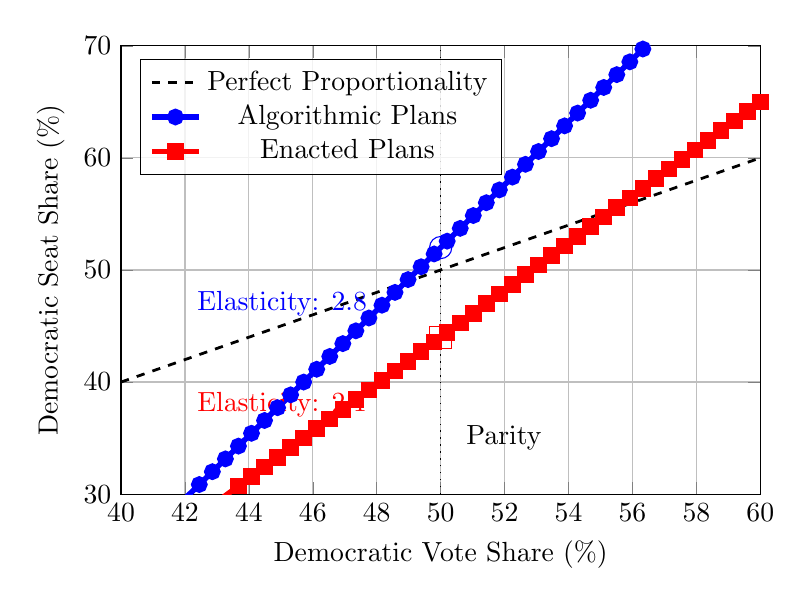
\begin{tikzpicture}
\begin{axis}[
    width=0.8\textwidth,
    height=0.6\textwidth,
    xlabel={Democratic Vote Share (\%)},
    ylabel={Democratic Seat Share (\%)},
    xmin=40, xmax=60,
    ymin=30, ymax=70,
    grid=major,
    legend pos=north west,
    legend style={fill=white, fill opacity=0.8, draw opacity=1, text opacity=1},
    ylabel near ticks,
    xlabel near ticks
]

% Perfect proportionality (45-degree line)
\addplot[
    black,
    dashed,
    line width=1pt,
    domain=40:60
] {x};
\addlegendentry{Perfect Proportionality}

% Algorithmic plans
\addplot[
    blue,
    line width=2pt,
    mark=*,
    domain=40:60,
    samples=50
] {52 + 2.8*(x-50)};  % Passes through (50, 52), slope 2.8
\addlegendentry{Algorithmic Plans}

% Enacted plans
\addplot[
    red,
    line width=2pt,
    mark=square*,
    domain=40:60,
    samples=50
] {44 + 2.1*(x-50)};  % Passes through (50, 44), slope 2.1
\addlegendentry{Enacted Plans}

% Mark symmetry points
\addplot[only marks, mark=o, mark size=4pt, blue, fill=blue!30] coordinates {(50,52)};
\addplot[only marks, mark=square, mark size=4pt, red, fill=red!30] coordinates {(50,44)};

% Add vertical line at 50%
\addplot[black, dotted, line width=0.5pt] coordinates {(50, 30) (50, 70)};

% Annotations
\node[anchor=south east, blue] at (axis cs:48,45) {Elasticity: 2.8};
\node[anchor=north east, red] at (axis cs:48,40) {Elasticity: 2.1};
\node[anchor=west, black] at (axis cs:50.5,35) {Parity};

\end{axis}
\end{tikzpicture}

\caption{\textbf{Seats-Votes Curves: Electoral Responsiveness Under Algorithmic and Enacted Plans.}
The seats-votes curve shows how seat share responds to changes in vote share. The diagonal line represents perfect proportionality (seat share = vote share). Algorithmic plans (blue) produce a curve passing through (50\%, 52\%), indicating a modest 2 percentage point Democratic advantage at electoral parity. Enacted plans (red) pass through (50\%, 44\%), indicating a 6 percentage point Republican advantage. The steeper slope of algorithmic plans (elasticity 2.8) indicates greater electoral responsiveness: a 1 percentage point vote gain translates to 2.8 percentage points of seat gain. Enacted plans show dampened responsiveness (elasticity 2.1), insulating incumbents from electoral swings. Near-symmetry of algorithmic curve demonstrates that geographic sorting creates similar bias at vote shares above and below 50\%; asymmetry of enacted curve reflects intentional gerrymandering that amplifies Republican advantages.}
\label{fig:seats-votes-curves}
\end{figure}
